\documentclass[titlepage]{article}
\usepackage[utf8]{inputenc}
\usepackage{graphicx}
\usepackage{afterpage}
    \newcommand\blankpage{
    \null
    \thispagestyle{empty}
    \addtocounter{page}{-1}
    \newpage
    }
\usepackage[
backend=biber,
style=numeric,
sorting=none
]{biblatex}
\addbibresource{References.bib}
\title{NANOGRID FOR RENEWABLE OFF-GRID SYSTEM}
\author{Onyia Chukwuebuka Louis }
\date{September, 2019}
\begin{document}
    \afterpage{\blankpage}
    \maketitle
    \afterpage{\blankpage}
    \begin{abstract}
    Power grids utilize large central generating stations which entails the use of long transmission lines to deliver power to consumers. This approach poses some challenges such as line loses, carbon dioxide ($CO_{2}$) emission into the environment from the burning of fossil fuels from such large generators and also, little or no availability of electricity in the rural and isolated areas where the supply of power from the national grid may be considered uneconomical. Distributed generation proffers solutions to these challenges by generating power close to the point of consumption. A nanogrid is an important aspect of distributed generation in which electricity is generated for a single building. Nanogrids usually employ renewable sources of power such as solar and wind energy to generate electricity, hence reducing carbon dioxide emission. Also due to the versatility of nanogrids, people in the rural areas can generate their own electricity. However, the intermittent supply of power due to the variations of wind speed during the entire course of a day poses a major challenge in the use of nanogrids. This thesis focuses on the study of the interaction of the savonius wind turbine in an existing nanogrid with a particular load so as to have a better understanding of how the wind turbine parameters such as the wind speed and TSR can affect the power generated from the turbine.This is achieved by modeling and measuring the power absorbtion of the savonius wind turbine operating in the nanogrid. 
    \paragraph{}From the results obtained in this project, it is glaring that the wind speed and Tip Speed Ratio of the wind turbine play a vital role in the total power harvested from the turbine. If the rotor blades spin too slowly, the wind will pass through the gap between the blades and no power will be generated. Whereas when the blades spin too fast, they act like a shield against the wind speed, creating turbulence in the air as they spin and so when the incoming blade arrives too fast, it hits the turbulent air created by the blade before it and thus no power will also be generated in this situation. Therefore,  it is of utmost importance to design the wind turbine with an optimal Tip Speed Ratio to obtain maximum power from the turbine and thus, improve the reliability and efficiency of the nanogrid technology. 
    \end{abstract}
\tableofcontents
\clearpage
\addcontentsline{toc}{section}{List of figures}
\addcontentsline{toc}{section}{List of tables}
\listoffigures
\listoftables
\clearpage
\section{Introduction}
\paragraph{} The focus of this section is to give an insight into the background of the problem and the goals/objectives of this project.

\subsection{Background}
\paragraph{} The existing power infrastructures are currently facing some challenges which are partly due to the use of long distance transmission lines to deliver electricity from large central stations to consumers. These large central power generators are often fossil fuel based solutions contributing to the 30.8 billion tons of carbon dioxide released into the atmosphere each year~\cite{Friedlingstein}. This approach of power distribution causes significant line loses and adversely affects the grid's efficiency. Further more, it greatly affects people in the rural communities where the electricity generated from the grid may not be supplied to since it is perceived to be uneconomical.
\paragraph{}In a bid to solve these problems, there have been some on going research on distributed generation (DG) whereby power can be produced close to the point of consumption. By this approach, long distance power distribution can be avoided, and consequently, line loses and power outages are also minimized.  DG has a smaller power capacity than a central generation station which makes it a versatile power solution~\cite{Paliwal}. Hence, DG  makes it possible for power consumers to produce their own electricity for their residential or commercial property. This helps to improve the availability of electricity in the rural or isolated areas. It also provides security of supply, in the sense that even if power outage should occur at the national grid for any reason, some commercial and residential buildings which have operational nanogrids can still generate their own electricity and operate on islanded mode. In addition, DG often times but not always, employs renewable energy sources such solar and/or wind sources, thereby reducing the use of fossil fuels for electricity generation and consequently reducing the amount of $CO_{2}$ in the atmosphere. 
\paragraph{} One major draw-back of DG is its intermittent supply of power. The output power largely depends on wind speed (wind energy) and sun intensity (solar energy) leading to varying magnitude of output power during the entire day. These inadequacies can be addressed from a control system point of view,to optimize demand and supply~\cite{AghaeiJ}. A microgrid is a control system that combines various types of DG and optimize its use to meet the power demands of small communities, hospitals and university campuses ~\cite{PlanasE}. When we talk about the generation of electricity for a single home, then we refer to "Nanogrids" which is the focus of this project. It is a scaled-down version of microgrids. 

\subsection{Objective}
\paragraph{} The ultimate objective of this project is to model and measure the power absorbtion of Savounius Wind Turbine "Sawint" operating in the an existing nanogrid system. The turbine is made to supply a load and analysis carried out to ascertain how the wind speed and Tip Speed Ratio(TSR) affect the total power generated from the turbine and hence, apply the results obtained to future nanogrid projects, to develop a more reliable and efficient nanogrid technology.

\subsubsection{Goals}
\paragraph{} The goals of this thesis are listed below:
\begin{enumerate}
    \item Design a load circuit to interact with the savounius wind turbine in an existing nanogrid, and observe the operation of the nanogrid components when supplying power to the load at different wind speeds.
    \item Investigate how the wind speed and tip speed ratio (TSR) of the turbine affects the power output.
    \item Make recommendations for further studies based on obtained result 
\end{enumerate}

\clearpage
\section{Theory}
\subsection{Nanogrid}
\paragraph{}A nanogrid is simply a power distribution system, with the capability of operating in grid connected or islanded mode (when not connected to the grid).
It is a single domain for voltage, reliability and administration~\cite{Bruce}.
Nanogrids can also be concisely defined as a power distribution system for a single house or small building,with the ability to connect or disconnect from other power entities via a gateway.It consists of local power production powering local loads,with the option of utilising energy storage and/or a control system~\cite{Burmester}.

\begin{figure}[h!]
\centering
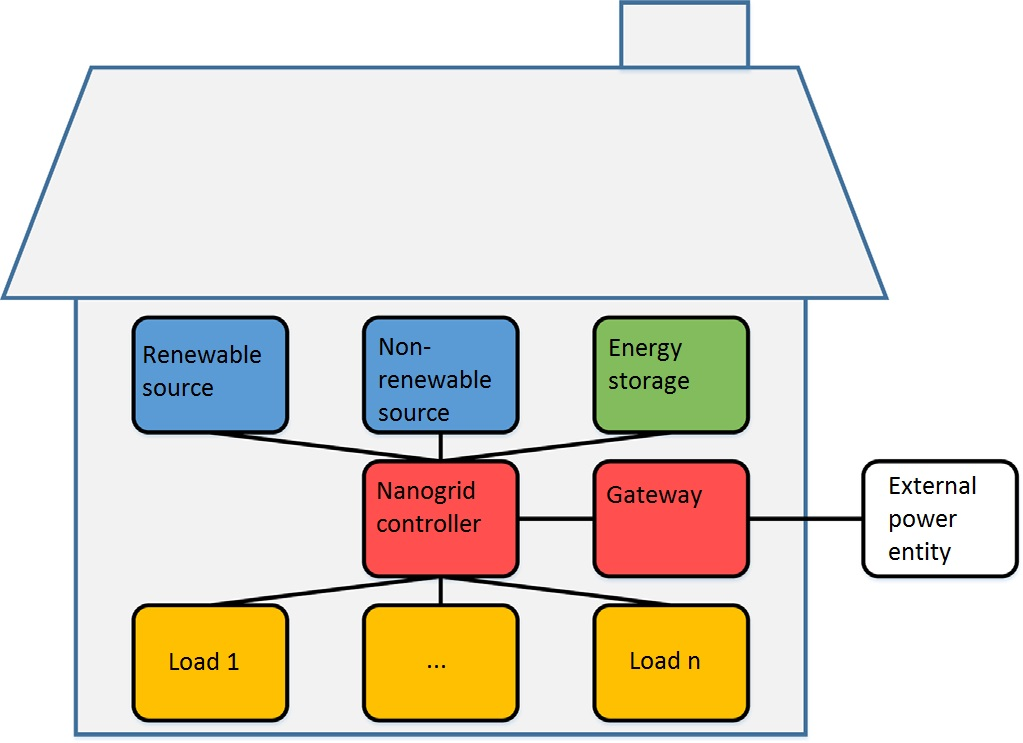
\includegraphics[scale=0.4]{Nanogrid.jpg}
\caption{Block diagram of a nanogrid}~\cite{Burmester}
\label{Nanogrid}
\end{figure}

\subsubsection{Components of a nanogrid}
\begin{enumerate}
    \item Local power production: This could be renewable energy sources such solar and wind power, and/or non-renewable energy sources such as diesel generators or fuel cells.
    \item Local load: There would be at least one local load that is being supplied power from the local power production. Local loads are household electrical appliances such as television, sound systems or ligting etc.
    \item Gateway: This is a bidirectional power connection between other nanogrids, microgrids or the national grid. This may also include communication with other power entities, conveying the nanogrids power requirements~\cite{Burmester}. Through the gateway, the nanogrid can also buy power from, and sell power to other connected power entities. It can also be disconnected from external power entities to allow the nanogrid operate in islanded mode. 
    \item Energy Storage: The most suitable energy storage for a nanogrid is a battery bank. Having an energy storage system is optional but it helps to add stability to the nanogrid.
    \item Nanogrid controller: This is the brain of the system, and provides the systems the ability to coordinate multiple sources and optimize power production and consumption. We have two types of nanogrid controllers; Central control and decentralized control. 
    \paragraph{}A central control comprises central controller that acts on information from sensors measuring the power control and consumption of the system. On the other-hand, a decentralized control comprises series of control nodes, operating independently to sense the status of each local source and load~\cite{Burmester}. A decentralized controller is more reliable and faster than a central controller. However, it is limited in its usefulness due to lack of communication between its system nodes.   
\end{enumerate}

\subsection{Wind turbine resource}
\paragraph{}A wind turbine converts the kinetic energy in the wind into mechanical energy of the rotor, this mechanical energy can then be converted into electrical energy by the use of a generator. When the wind flows across the blades of the turbine, this results in a decrease in air pressure on one side of the blade. The difference in air pressure between the two sides of the blade causes both lift and drag. However, the force from the lift and the drag makes the rotor spin. The rotor is connected to the generator either directly ( in the case of a direct drive turbine) or through a shaft and a gear box which speeds up the rotation. This conversion of aerodynamics force to rotation of a generator generates electricity. 

There are two types of wind turbines:
\subsubsection{Horizontal Axis Wind Turbine (HAWT)}These are the most commonly used wind turbines, and are made up a horizontal rotor shaft and an electrical generator. They usually have three blades and are operated upwind with the turbine pivoting at the top of the tower so the blades face into the wind~\cite{Energy.govwebsite}.
\subsubsection{Vertical Axis Wind Turbine (VAWT)}They are designed with a vertical rotor shaft, an electrical generator and gearbox which are placed at the bottom of the turbine, and a uniquely shaped rotor blade that is designed to harvest the power of the wind regardless of its direction~\cite{T.AI-Shemmeri}.
\paragraph{}There are two types of VAWTS; Savonius and Darrieus. The Darrieus turbine is driven by lift force on the blades, whereas the Savonius turbine is mostly driven by drag forces. The Savonius turbine used in the existing nanogrid for this project is called a SAWINT (Savonius Wind Turbine). It has a height of 2 meters and a diameter of 1 meter. 
\subsubsection{Wind speed of turbines}
\paragraph{} The wind speed of a turbine largely determines the electrical power output of the turbine. Higher wind speed result to faster rotation of the rotor, which translates to more mechanical power and more electrical power from the generator. However, turbines are designed to operate within a certain range of wind speed limits
\begin{enumerate}
    \item Start-up Speed: At this speed, the rotor and blade assembly begin to rotate.
    \item Cut-in speed: This is the minimum speed at which the turbine will begin to produce usable power. 
    \item Rated speed: This is the minimum speed at which the turbine will produce its designated rated power. Between the cut-in speed and the rated speed, the power generated by the turbine increases cubically with the wind speed.
    \item Cut out speed: This is the maximum wind speed beyond which the turbine would be shut-down. It's a safety feature which prevents the turbine from damage.
    
\begin{figure}[h!]
\centering
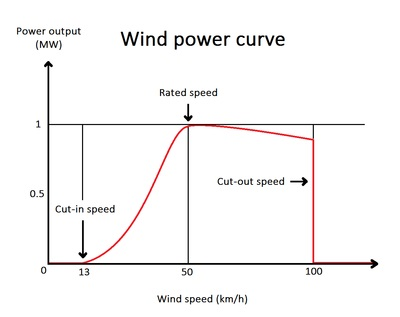
\includegraphics[scale=0.8]{Windspeedcurve.jpg}
\caption{Typical wind turbine power output with steady wind speed}~\cite{windpowerprogramwebsite}
\label{Windspeedcurve}
\end{figure}
    
\end{enumerate}
\subsection{Wind turbine design parameters}
\subsubsection{Tip Speed Ratio (TSR)} This is the ratio of the blade tip speed to the wind speed. It is an extremely important parameter in the design of a wind turbine. Expressed as 
\begin{equation}\label{}
    TSR(\lambda) = \frac{Blade tip speeed}{Wind speed}.
\end{equation}
    \paragraph{}Where blade tip speed is equal to the product of the rotational wind speed , $\omega$ (in radians/sec) and the radius, r. Expressed as 
\begin{equation}\label{}
    Bladetipspeed = \omega r.
\end{equation}
\paragraph{} If the rotor spins too slowly, most of the wind would pass through the gap between the blades without generating any power. If it spins too fast then the blades would act like a shield to the wind. Furthermore, rotor blades create turbulence as they spin through the air, so if the next blade arrives too quickly it would hit that turbulent air. Therefore, it is very important to design wind turbines with optimal TSR to achieve maximum amount of power.
\subsubsection{Power Coefficient $C_{p}$} This is the ratio of the power extracted by the turbine to the total power contained in the undisturbed cross-section. Expressed as 
\begin{equation}\label{}
 C_{p} = \frac{P_{T}}{P_{W}}.  
\end{equation}
\subsubsection{Swept Area } The swept area of the Savonis turbine is the product of the height of the blade and it's diameter. Expressed as $$A = h \times d (m^2).$$
\subsubsection{Turbine Power $P_{T}$ }  This is the power extracted by the turbine. Expressed as  
\begin{equation}\label{}
P_{T} = \frac{1}{2} \rho A V^3 C_{p}.
\end{equation}
    \paragraph{}where:
         $$ \rho = Air density $$
        $$V = Wind speed (m/s)$$
         $$ A = Swept area (m^2)$$
        $$ C_{p} = Power coefficient $$
    

\subsection{Power resource}
\subsubsection{Rectifier}

A rectifier is a circuit that is used to convert alternating current (AC) to direct current (DC). There are two types, half wave rectifiers and full wave rectifiers. On this project, a full wave rectification circuit was employed.


\subsubsection{Full wave rectifier}

\paragraph{}In this type of rectification, there is a flow of current through the load both in the negative and positive half-cycles of the input AC voltage. To achieve this, two diodes work alternately. In the positive half-cycle of the AC voltage, the first diode which is forward biased supplies the load while in the negative half-cycle of the AC voltage, the second diode which is reverse biased supplies the load. There are two types of full wave rectifiers:
\begin{enumerate}
  \item Center-tapped full wave rectifier
  \item Full wave bridge rectifier
 \end{enumerate} 
  
\paragraph{ } On this project, we utilized a full wave bridge rectifier circuit. The circuit contains four diodes $ D_{1}, D_{2}, D_{3} and D_{4} $, connected to form a bridge as shown in figure 3 below. The AC supply to be rectifier is applied to the diagonally opposite ends of the bridge through the transformer. Between the other two ends of the bridge, the load resistance $ R_{L} $ is connected ~\cite{MEHTA}

\paragraph{}During the positive half cycle of the input voltage, the upper end of the transformer secondary winding is made positive with respect to the lower end. consequently, diodes $D_{1}$ and $D_{3}$ are forward biased while diodes $D_{2}$ and $D_{4}$ are reverse biased. As a result, current flows across the load $R_{L}$ through $D_{1}$ and $D_{3}$ only. During the negative half of the input voltage, the lower end of the transformer secondary winding is made positive with respect to the upper end. Thus, diodes $D_{2}$ and $D_{4}$ are forward biased while $D_{1}$ and $D_{3}$ are reverse  biased. As a result, diodes $D_{2}$ and $D_{4}$ conduct current through the load $R_{L}$ as shown in figure 3 below.
\begin{figure}[h!]
\centering
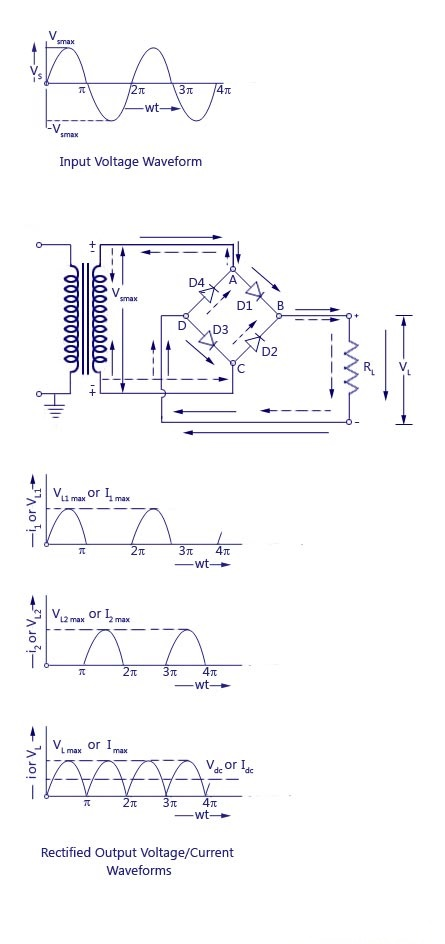
\includegraphics[scale=0.7]{bridge_rectifier.jpg}
\caption{Full wave bridge rectifier
circuit}~\cite{Circuitstodaywebsite}
\label{bridge_rectifier}
\end{figure}
\clearpage
\subsubsection{Capacitor}
\paragraph{} On this project, a capacitor is basically  used for smoothing the output voltage from the full wave rectifier so as to obtain a DC supply with a smooth and constant output voltage. This is because the voltage from the full wave rectifier is always pulsating. This is shown in the figure 4 below.

\begin{figure}[h!]
\centering
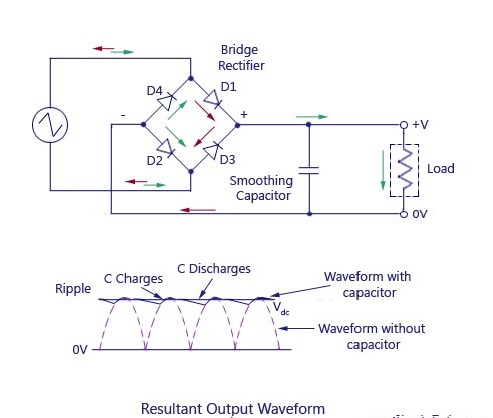
\includegraphics[scale=0.7]{bridge_rectifier_with_capacitor_filter.jpg}
\caption{Full wave bridge rectifier with capacitor filter}~\cite{Circuitstodaywebsite}
\label{bridge_rectifier_with_capacitor_filter}
\end{figure}

\subsubsection{Zener diode}
\paragraph{} A Zener diode conducts current when it is reverse biased unlike a regular diode that only allows the flow of current when it is forward biased. When the reverse voltage applied across the Zener diode exceeds the rated voltage of the device a process called "Avalanche Breakdown" occurs in the semiconductor depletion layer and a current starts to flow through the diode to limit this increase in voltage. As seen on the I-V characteristics shown in figure 5, the Zener diode has a region in its reverse bias characteristics where the negative voltage remains almost constant regardless of the value of current flowing through the diode, as long as the zener diode current remains between the breakdown current $I_{Z}$ and the maximum current rating $I_{Z(max)}$. 

\begin{figure}[h!]
\centering
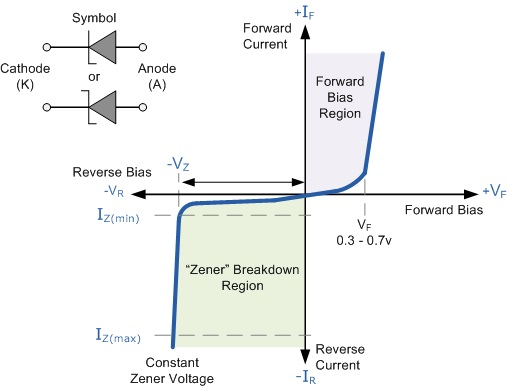
\includegraphics[scale=0.8]{Zener-diode11.jpg}
\caption{Zener diode I-V Characteristics}~\cite{Electronicstutorialwebsite}
\label{Zener-diode11}
\end{figure}
\clearpage
\section{Method}
\subsection{Design and construction of load circuit}
\paragraph{}I started out by designing the load circuit on Pspice. As seen on figure 6 below, it consist of two full wave rectifiers, to rectify the AC input from the generator to DC. There is also a 10 mF capacitor connected in parallel for smoothing the DC supply.  Twelve Zener diodes $ D_1 $ through $ D_{12} $, each connected in series with a 4 ohm power resistor and also connected in parallel branches to one another to ensure that non of them exceeded the maximum rated power. The zener diodes have a reverse breakdown voltage of 16 V. The resistors in series with the zener diodes do not only help to dissipate power but also to distribute current evenly between the parallel connected zener diodes. 
\begin{table}[h]
\centering
\begin{tabular}{ |c|c|c| } 
 \hline
 Component & value & Quantity \\ 
 \hline
 Zener diodes & 16 V & 12 \\ 
 Power Resistors & 4 Ohm & 12 \\
 Capacitor & 10 mF & 1\\
 \hline
\end{tabular}
\caption{List of components}
\label{table:1}
\end{table}

\begin{figure}[h]
\centering
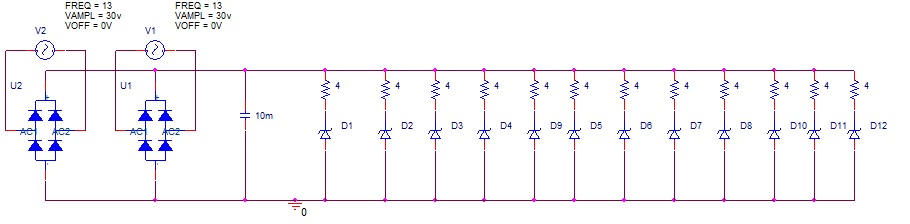
\includegraphics[scale=0.6]{Loadcct.jpg}
\caption{Load Cicuit as designed on Pspice}
\label{Loadcct}
\end{figure}

\begin{figure}[h]
\centering
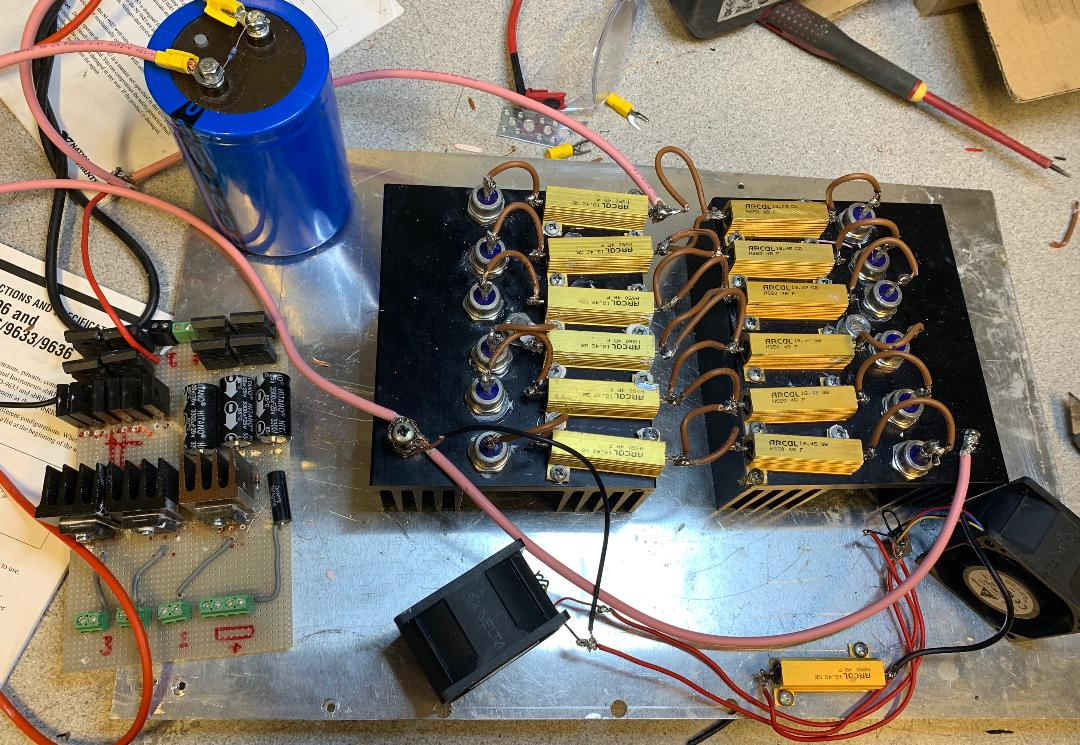
\includegraphics[scale=0.3]{realcct.jpg}
\caption{Actual load circuit}
\label{constructed load cct}
\end{figure}
\clearpage
\subsection{Calculation of turbine parameters}
From measurements gotten from the existing turbine data, Time period of rotation of turbine blade, $T_{p} = 0.07802~s$ 
\paragraph{} Frequency of rotation, $F = \frac{1}{T_{p}}$ $$F = \frac{1}{0.07802} = 12.82~Hz$$
 Revolution per minute(RPM) $ = \frac{F}{No. of poles}\times60 $
\begin{equation}\label{}
RPM = \frac{12.82}{7} \times60 = 109.87~rev/min
\end{equation}
rotational speed,
\begin{equation}\label{}
\omega = \frac{109,87}{60}\times2 \pi = 11.51~rad/sec
\end{equation}
I determined the value of the constant "K", from the formular 
\begin{equation}\label{}
K = \frac{v}{\omega},
\end{equation}
where $\omega = Rotational speed (rad/s) $ and v = voltage
\paragraph{}From measurements, $\omega = 11.51~rad/s$ and $ v = 31.28~V$
\begin{equation}\label{}
K = \frac{31.28}{11.51} = 2.72 
\end{equation}
The idea is to get the different rotational speeds at which the electrical power consumption at the load is equal to the mechanical power production of the turbine in the existing nanogrid. When the power consumption at the load is greater than the generated turbine power  then the frequency of rotation will reduce but if the power consumption of the load is less than the power generation of the turbine, the frequency of the turbine increases.  

Based on data gotten from actual measurements of the turbine parameters,I calculated the initial angular speed to be 11.51~rad/s as shown on equation (6) above. I then started with a rough guess and carried out several iterations until I got the different angular speeds where the mechanical power of the turbine is equal to the electrical power consumed at the load.
\subsubsection{Pspice simulations}
First on the Pspice software, I varied the input voltage from 16~V through 30~V and calculated the maximum power output for each case. The relationship between power and voltage is given by 
\begin{equation}\label{}
P = IV~(W)
\end{equation}
\paragraph{} The same voltage would flow through the 12 branches on the load circuit, since voltage is the same for parallel connections whereas the current through the various branches would vary. This is based on ohms law 
\begin{equation}\label{}
V = IR~(V)
\end{equation}
\begin{equation}\label{}
I = \frac{V}{R}~(A)
\end{equation}
Therefore, for each input voltage, the total power at the load is calculated by summing the current available on each branch, and then multiplying the total sum of current values with the input voltage.
\begin{figure}[h!]
\centering
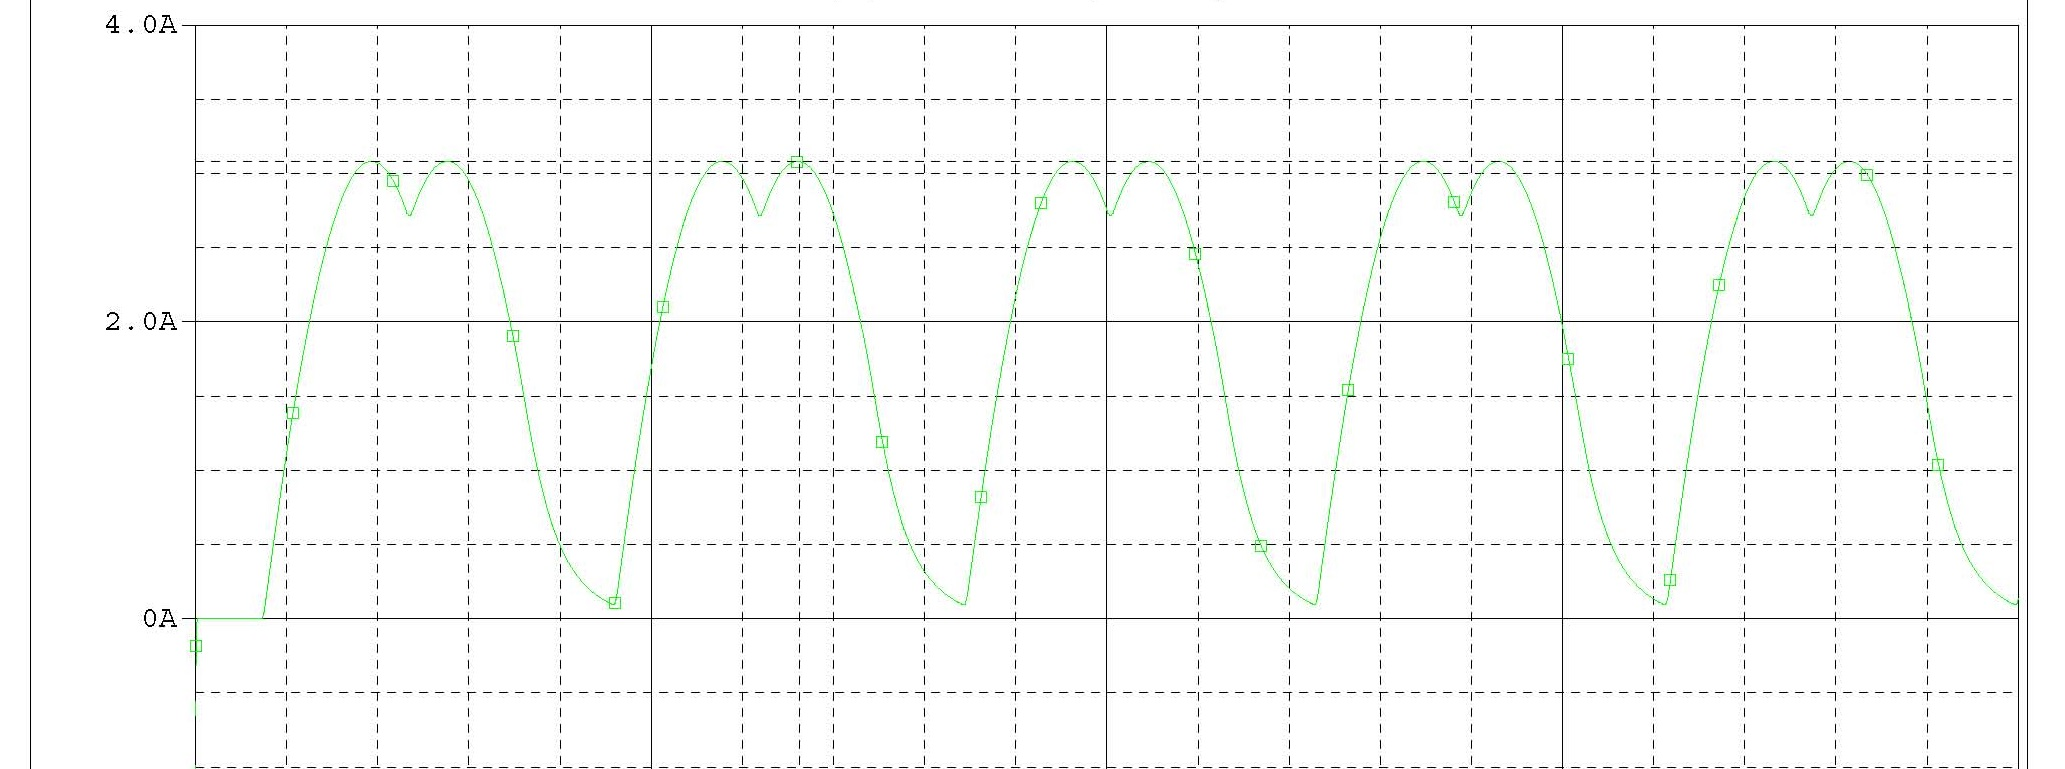
\includegraphics[scale=0.5]{pspice1.jpg}
\caption{Pspice simulation for maximum current value at load branch}
\label{pspice1}
\end{figure}
For instance, figure 7 below shows the simulation for the value of the current at one of the parallel branches when 30V was supplied at the input. From the simulation, is it seen that with a supply of 30V, a maximum current value of 3.08A was obtained at one of the parallel load branches. So the total maximum current would be $$ I = 3.08 \times 12 = 36.96~A$$ and the corresponding maximum output power is $$  P = 36.96 \times 30=~1.1~KW. $$
\paragraph{}This approach was repeated for input voltages of 16 V through 30 V and the results obtained is shown on the subsequent section.
\clearpage
\section{Results}
\subsubsection{Pspice simulation result}
Table 2 below shows the corresponding electrical output power for input voltages of 16~V through 30~V, as obtained from my Pspice simulation. 
\begin{table}[h!]
\centering
\begin{tabular}{ |c|c|} 
 \hline
 Power (W) & Voltage (V)\\
\hline
0 &	16\\
0.0127 & 17\\
0.0585 & 18\\
0.1128 & 19\\
0.1737 & 20\\
0.2408 & 21\\
0.3139 & 22\\
0.3929 & 23\\
0.4777 & 24\\
0.5684 & 25\\
0.665  & 26\\
0.7673 & 27\\
0.8754 & 28\\
0.9893 & 29\\
1.109  & 30\\
 \hline
\end{tabular}
\caption{Electrical power output for various input voltages, as obtained from Pspice simulation}
\label{table:1}
\end{table}

The result shows that as the generated voltage increases, the corresponding output power also increases.
\begin{figure}[h!]
\centering
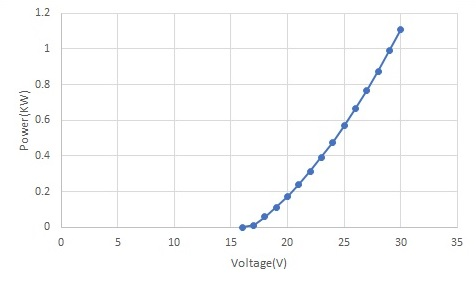
\includegraphics[scale=0.8]{voltageVSpower.jpg}
\caption{Relationship between the input voltage and the electrical power output}
\label{voltageVSpower}
\end{figure}
\paragraph{}From the available turbine measurements and calculations, the various parameters for the turbine and load are derived.
\begin{table}[h!]
\centering
\begin{tabular}{ |c|c|c|c|c|c|c|c| } 
 \hline
w (rad/s) & $V_{wind}(m/s)$ & Vgen(v) & BTS & TSR & Cp & $P_{turbine}$(W)& $P_{load}(W)$\\
\hline
5.5800& 3&  15.1664&    2.7900& 0.9300& 0.7448& 12&     12\\
6.0347&	4&	16.4004&	3.0170&	0.7543&	0.5548&	21&	    21\\
6.2500& 5&	16.9875&	3.1250&	0.6250&	0.4305& 31&	    31\\
6.459&	6&	17.5556&	3.2295&	0.5383&	0.3542&	45&	    45\\
6.653&	7&	18.0828&	3.3265&	0.4752&	0.3022&	60&	    60\\
6.854&	8&	18.6292&	3.4270&	0.4284&	0.2656&	79&	    79\\
7.055&	9&	19.1755&	3.5275&	0.3919&	0.2381&	101&	101\\
7.256&	10&	19.7218&	3.6280&	0.3628&	0.2168&	126&	126\\
7.46&	11&	20.2763&	3.7300&	0.3391&	0.1999&	155&	155\\
7.46&	12&	20.8471&	3.8350&	0.3196&	0.1863&	188&	188\\
7.88&	13&	21.4178&	3.9400&	0.3031&	0.1750&	224&    224\\
8.095&	14&	22.0022&	4.0475&	0.2891&	0.1656&	265&    265\\
8.309&	15&	22.5839&	4.1545&	0.2770& 0.1575&	310&	310\\
8.527&	16&	23.1764&	4.2635&	0.2665&	0.1506&	359&	359\\
8.755&	17&	23.7961&	4.3775&	0.2575&	0.1448&	414&	414\\
8.99&	18&	24.4348&	4.4950&	0.2497&	0.1397&	475&	475\\
9.227&	19&	25.0789&	4.6135&	0.2428&	0.1353&	541&	541\\
9.47&	20&	25.7394&	4.7350&	0.2368&	0.1315&	613&	613\\
9.715&	21&	26.4053&	4.8575&	0.2313&	0.1280&	691&	691\\
9.969&	22&	27.0957&	4.9845&	0.2266&	0.1250&	776&	776\\
10.227&	23&	27.7970&	5.1135&	0.2223&	0.1224&	868&	868\\
10.49&	24&	28.5118&	5.2450&	0.2185&	0.1200&	967&	967\\
10.76&	25&	29.2457&	5.3800&	0.2152&	0.1179&	1074&	1074\\
11.035&	26&	29.9931&	5.5175&	0.2122&	0.1161&	1189&	1189\\
11.316&	27&	30.7569&	5.6580&	0.2096&	0.1145&	1313&	1313\\
11.604&	28&	31.5396&	5.8020&	0.2072&	0.1130&	1446&	1446\\
11.896&	29&	32.3333&	5.9480&	0.2051&	0.1117&	1588&	1588\\
12.197&	30&	33.1515&	6.0985&	0.2032&	0.1106&	1741&	1741\\
\hline
\end{tabular}
\caption{Comparing the turbine power and electrical power}
\label{table:1}
\end{table}
\paragraph{}As shown on tables 3 above, for each wind speed $V_{wind}$ there is a generated voltage $V_{gen}$ which is the product of the rotational speed $\omega$ and the constant K as obtained in equation (8). That is, 
\begin{equation}\label{}
V_{gen} = \omega K.
\end{equation}
\paragraph{}The blade Tip Speed (BTS) as explained on equation (2) is the product of the rotational speed and the radius of the blade (which in this case is 0.5). From the calculated BTS, the Tip Speed ratio (TSR) can then be calculated using equation (1), by dividing the BTS by the wind speed value. The power coefficient is then calculated with the formular 
\begin{equation}\label{}
C{p} = (0.57 \times TSR) + (0.375 \times TSR^2) + (0.04 \times TSR^3) \times 0.84
\end{equation}
With the calculated value of $C_{p}$, the power generated from the turbine can then also be calculated using equation (4). Finally, I started my iteration with an initial guess of about half the value of the rotational speed obtained in equation (6) which is about 5.75 rad/s for the lowest wind speed of 3 m/s. I then continued varying the value of the rotational speed around that range until the power of the turbine generated is equal to the electrical power absorbed by the load. I repeated the same approach for the subsequent wind speeds, as I increase the rotational speed correspondingly. 

\paragraph{} The final result as shown on table 3 above shows that if the rotational speed is too low, the rotor blades spin too slowly and most of the wind would pass straight through the gap between the blades. No useful power can be generated by the turbine in this situation. This is confirmed by the values in the table,For instance,  when the wind speed was 3m/s, we had a low rotational speed, and a low power of 12 W was generated by the turbine. Whereas at a high wind speed, for instance when we had a wind speed of 25 m/s, we had a high rotational speed and the speed of the rotor was just sufficient enough to generate useful power of about 1~KW. In a situation where the rotor blades spin too fast, the blades would  act like a shield against the wind and since rotor blades create turbulence when they spin, the next blade would arrive too fast and hit the turbulence generated by the blade before it. Hence, low or no power will be generated. Therefore, it is necessary for the wind turbine to be designed with an optimal TSR ratio where the rotation of the rotor blades is optimal for maximum mechanical power generation from the wind turbine.

\subsubsection{TSR as a function of wind speed}
From the calculated data in Table 3 above, it is seen that as the wind speed increases, the TSR decreases.At the highest wind speed of 25~m/s, we had the lowest TSR of 0.22, whereas at the lowest wind speed of 3 m/s we had the highest TSR of 0.93.
\begin{figure}[h!]
\centering
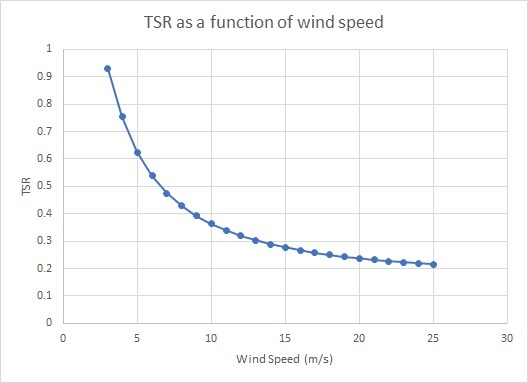
\includegraphics[scale=0.8]{TSR.jpg}
\caption{TSR as a function of wind speed}
\label{TSR}
\end{figure}

\subsubsection{Generated voltage as a funtion of wind speed}
From the data obtained in Table 3 above, it is also seen that as the wind speed increases, the voltage generated from the turbine also increases. At a low wind speed of 3~m/s, we had the lowest voltage of 15.2~V, whereas at a high wind speed of 25~m/s we had a high voltage of 29.2~V. This is shown on the graph below.

\begin{figure}[h!]
\centering
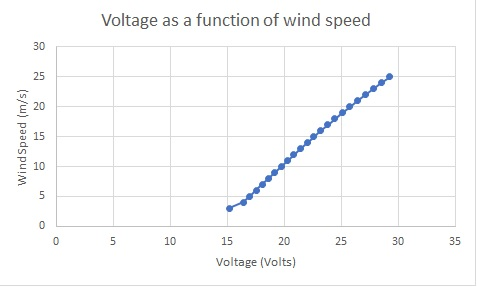
\includegraphics[scale=1]{vgen.jpg}
\caption{Voltage as a function of wind speed}
\label{Vgen}
\end{figure}

\subsubsection{Relationship between the rotational speed and the turbine power}
As the rotational speed increases, the mechanical power generated by the turbine also increases until it gets to its maximum power output. The power produced is limited to avoid overloading of the wind turbine.

\begin{figure}[h!]
\centering
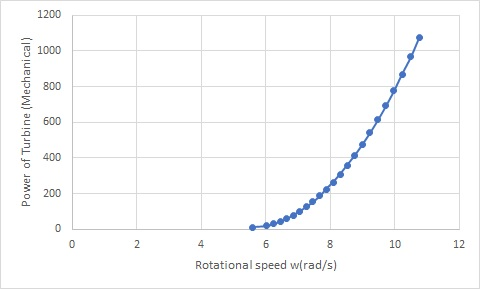
\includegraphics[scale=1]{turbinepower.jpg}
\caption{Relationship between the rotational speed and the mechanical turbine power}
\label{turbinepower}
\end{figure}
\clearpage
\section{Conclusion and future work}

\paragraph{}The results obtained from the interaction of the wind turbine and the designed load proves that, the wind speed and TSR greatly affect the mechanical power generated by the turbine. When the rotor blades spin too slowly, the wind will pass through the gaps between the blades and no power will be generated. whereas when the  blades spin too fast, they create turbulent air and if the incoming blade arrive too quickly it will then hit that turbulent air created by the blade before it and no power will be harvested from the wind. Thus, wind turbines must be designed with optimal TSR to generate maximum power from the turbine. 
\paragraph{} An optimal TSR ratio for a wind turbine can be calculated from the formula
\begin{equation}\label{}
\lambda(Max power) = \frac{4 \pi}{n} 
\end{equation}
where n = number of blades
\paragraph{} If the TSR is equal to 1, that means the blades are rotating at same speed as the wind speed. If the TSR is morethan 1, that means there is a lift involved which makes the rotor blades spin faster than the wind speed. However, a TSR less than 1 means that there is a lot of drag going on, which makes the blades spin slower than the wind speed. The rotation of the rotor blades can be slowed down by the amount of power consumed by the connected load. When the power consumed by the load is greater than the generated turbine power, the rotational speed decreases, but when the power generated by the turbine is greater than the power absorbed by the load, the rotational speed increases. Thus, it is of great importance to utilize a rotational speed where the power generated from the turbine is at a balance with the power absorbed by the load for a reliable and efficient operation of the nanogrid.

\paragraph{} Equipped with the knowlegde obtained from the analysis of this project, we can be able to optimize the wind turbine parameters such as rotational speed and TSR, so as to maximize power output of the turbine. This would help to improve the reliability and efficiency of the nanogrid. 

\paragraph{} Due to time constraints, I was unable to connect the load I built to the turbine in real life. The results I obtained from this project were mostly from simulations and calculations. For future work purpose, it would be interesting to connect the constructed load to the existing nanogrid and see how the load works in real life. 
 
\clearpage
\addcontentsline{toc}{section}{References}
\printbibliography
\end{document}
